\documentclass[12pt,frenchb]{beamer}
\usepackage[utf8]{inputenc}
\usepackage[T1]{fontenc}
%\usepackage{ntheorem}
\usepackage{amsmath}
\usepackage{amsfonts}

\usepackage{array}

\usepackage{kpfonts}


%\pdfminorversion 7
%\pdfobjcompresslevel 3

\usepackage{tabularx}

\usepackage{pgf}
\usepackage{tikz}
\usepackage{tkz-euclide}
\usetkzobj{all}
\usetikzlibrary{patterns}


\usepackage{lastpage}

\usepackage{marginnote}

\usepackage{wrapfig}
\usepackage{babel}

\usepackage[autolanguage]{numprint}
\newcommand{\np}{\numprint}

\makeatletter

\pgfdeclarepatternformonly{mes_hachures}
{\pgfpoint{-0.1cm}{-0.1cm}}
{\pgfpoint{0.9cm}{0.5cm}}
{\pgfpoint{0.8cm}{0.4cm}}
{\pgfpathmoveto{\pgfpointorigin}
  \pgfpathlineto{\pgfpoint{0.8cm}{0.4cm}}
\pgfusepath{stroke}}

\newcommand{\R}{\mathbf{R}}
\newcommand{\N}{\mathbf{N}}
\newcommand{\Vecteur}{\overrightarrow}
\newcommand{\norme}[1]{\left\lVert #1 \right\rVert}
\newcommand{\vabs}[1]{\left\lvert #1 \right\rvert}
\newcommand{\inff}[2]{\left[#1~;~#2\right]}
\newcommand{\info}[2]{\left[#1~;~#2\right[}
\newcommand{\inof}[2]{\left]#1~;~#2\right]}
\newcommand{\inoo}[2]{\left]#1~;~#2\right[}

\makeatother


\usepackage{multicol}
\setlength{\columnseprule}{0pt}

\everymath{\displaystyle\everymath{}}

\title{Fonction continue}
\author{Terminale S}
\institute{\bsc{LaSalle Saint-Denis}}
\date{octobre 2017}

\begin{document}

\begin{frame}
  \maketitle
\end{frame}

\section{Généralités}

\subsection{Définition}

\begin{frame}
  \begin{block}{}
      \begin{definition}
        Une fonction est dite \alert{continue} en $x_0$, si pour tout
        intervalle autour de $f(x_0)$, il existe un intervalle tel que
        toutes les images de cet intervalle sont dans l'intervalle autour de
        $f(x_0)$.
      \end{definition}
    \end{block}
\end{frame}

\begin{frame}
  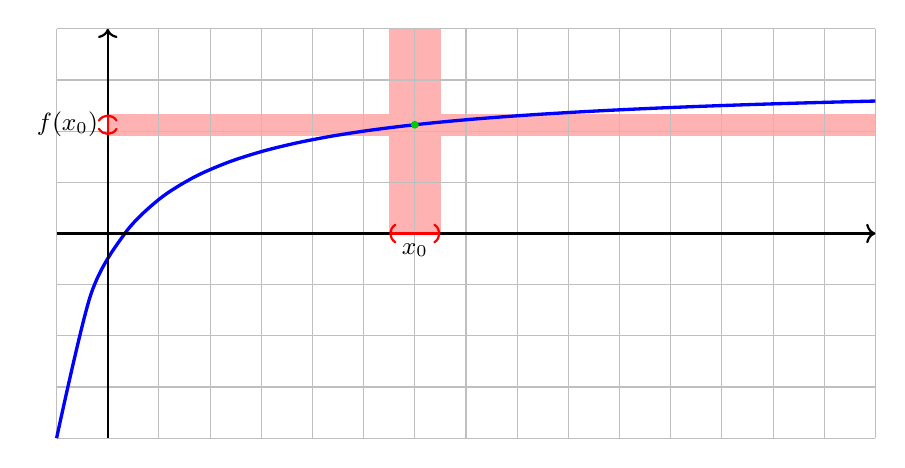
\begin{tikzpicture}[scale=0.65]
    \draw [red!30,fill=red!30] (6-0.5,0) rectangle (6+0.5,4) ;
    \draw [red!30,fill=red!30] (0,{(3*6-1)/(6+2) - 0.2}) rectangle
      (15,{(3*6-1)/(6+2) + 0.2}) ;
    \draw [thin, lightgray] (-1,-4) grid [step=1] (15,4) ;
    \draw [very thick, blue] plot [domain = -1:15,smooth]
    (\x,{(3*\x-1)/(\x+2)}) ;
    \draw [thick,->] (-1,0) -- (15,0) ;
    \draw [thick,->] (0,-4) -- (0,4) ;
    \draw (6,{(3*6-1)/(6+2)}) node
      [circle, fill, green!79!black, inner sep=1.0pt] {} ;
      \draw (6,{(3*6-1)/(6+2)});
    \draw [(-),red,thick] (6-0.5,0) -- (6+0.5,0) ;
    \draw [red,thick,(-)] (0,{(3*6-1)/(6+2) - 0.2}) --
      (0,{(3*6-1)/(6+2) + 0.2}) ;
    \draw (6,0) node [below ] { \small $x_0$ } ;
    \draw (0,{(3*6-1)/(6+2)}) node [left] { \small $f(x_0)$ } ;
  \end{tikzpicture}
\end{frame}

\begin{frame}
  \begin{block}{}
    \begin{definition}
      On dit qu'une fonction est continue sur un intervalle $I$, si elle est
      continue en chacun des points de l'intervalle.
    \end{definition}
      \begin{itemize}
        \item la somme (algébrique) et la multiplication par un réel
          conservent la continuité
        \item le produit de deux fonctions continues est continues
        \item si $f$ est dérivable sur $I$, $f$ est continue sur $I$.
      \end{itemize}
      Attention, la réciproque est fausse : $f : x \mapsto \sqrt{x}$ est
      continue sur $\info{0}{+\infty}$ et dérivable sur $\inoo{0}{+\infty}$.
  \end{block}
\end{frame}

\section{Le théorème des valeurs intermédiaires}

\subsection{TVI}

\begin{frame}
  \begin{block}{}
    \begin{theorem}[des valeurs intermédiaires]
      Soit $f$ une fonction continue sur un intervalle $I$. Alors
      \begin{itemize}
        \item $f(I)$ est un intervalle ;
        \item pour tout $k \in f(I)$, l'équation $f(x) = k$ admet au moins
          une solution.
      \end{itemize}
    \end{theorem}
  \end{block}
\end{frame}


\subsection{Corollaire}

\begin{frame}
  \begin{block}{}
    \begin{theorem}[corollaire du précédent]
      Soit $f$ une fonction continue sur un intervalle $I = [a;b]$,
      \alert{strictement monotone}. Alors
      \begin{itemize}
        \item $f(I) = [f(a);f(b)]$ pour une fonction croissante est un
          intervalle ;
        \item pour tout $k \in f(I)$, l'équation $f(x) = k$ admet exactement
          \alert{une et une seule} solution.
      \end{itemize}
    \end{theorem}
  \end{block}
\end{frame}


\end{document}
